\chapter{Implementation}
\graphicspath{{Chapter4/Figs/}{Chapter4/Figs/}}

This chapter goes into the implementation details of building the software parts for the NIP of IDUN and the key events that occurred during this empirical software engineering process, such as the realisation of the novelty and the need for a definition for a N/CI. Next to that, the author also discusses other key aspects and learnings from building the system.

\section{Timeline}
\label{chapter4-timeline}

Procedures, such as enlisted in the project stages presented in \autoref{chapter3-project-stages}, are a good guide for project implementation, but in the end, such plans run in unexpected ways. As a result, researching and implementing a non-trivial system such as a N/CI requires a high level of agility.

The effective timeline at the time of writing is shown in \autoref{fig:implementation-timeline}. It includes the previously mentioned project stages but is differently structured as initially described. \autoref{tab:special-project-stages} explains why some project stages were completed differently than initially planned.

\begin{figure}[!ht]
  \centering
  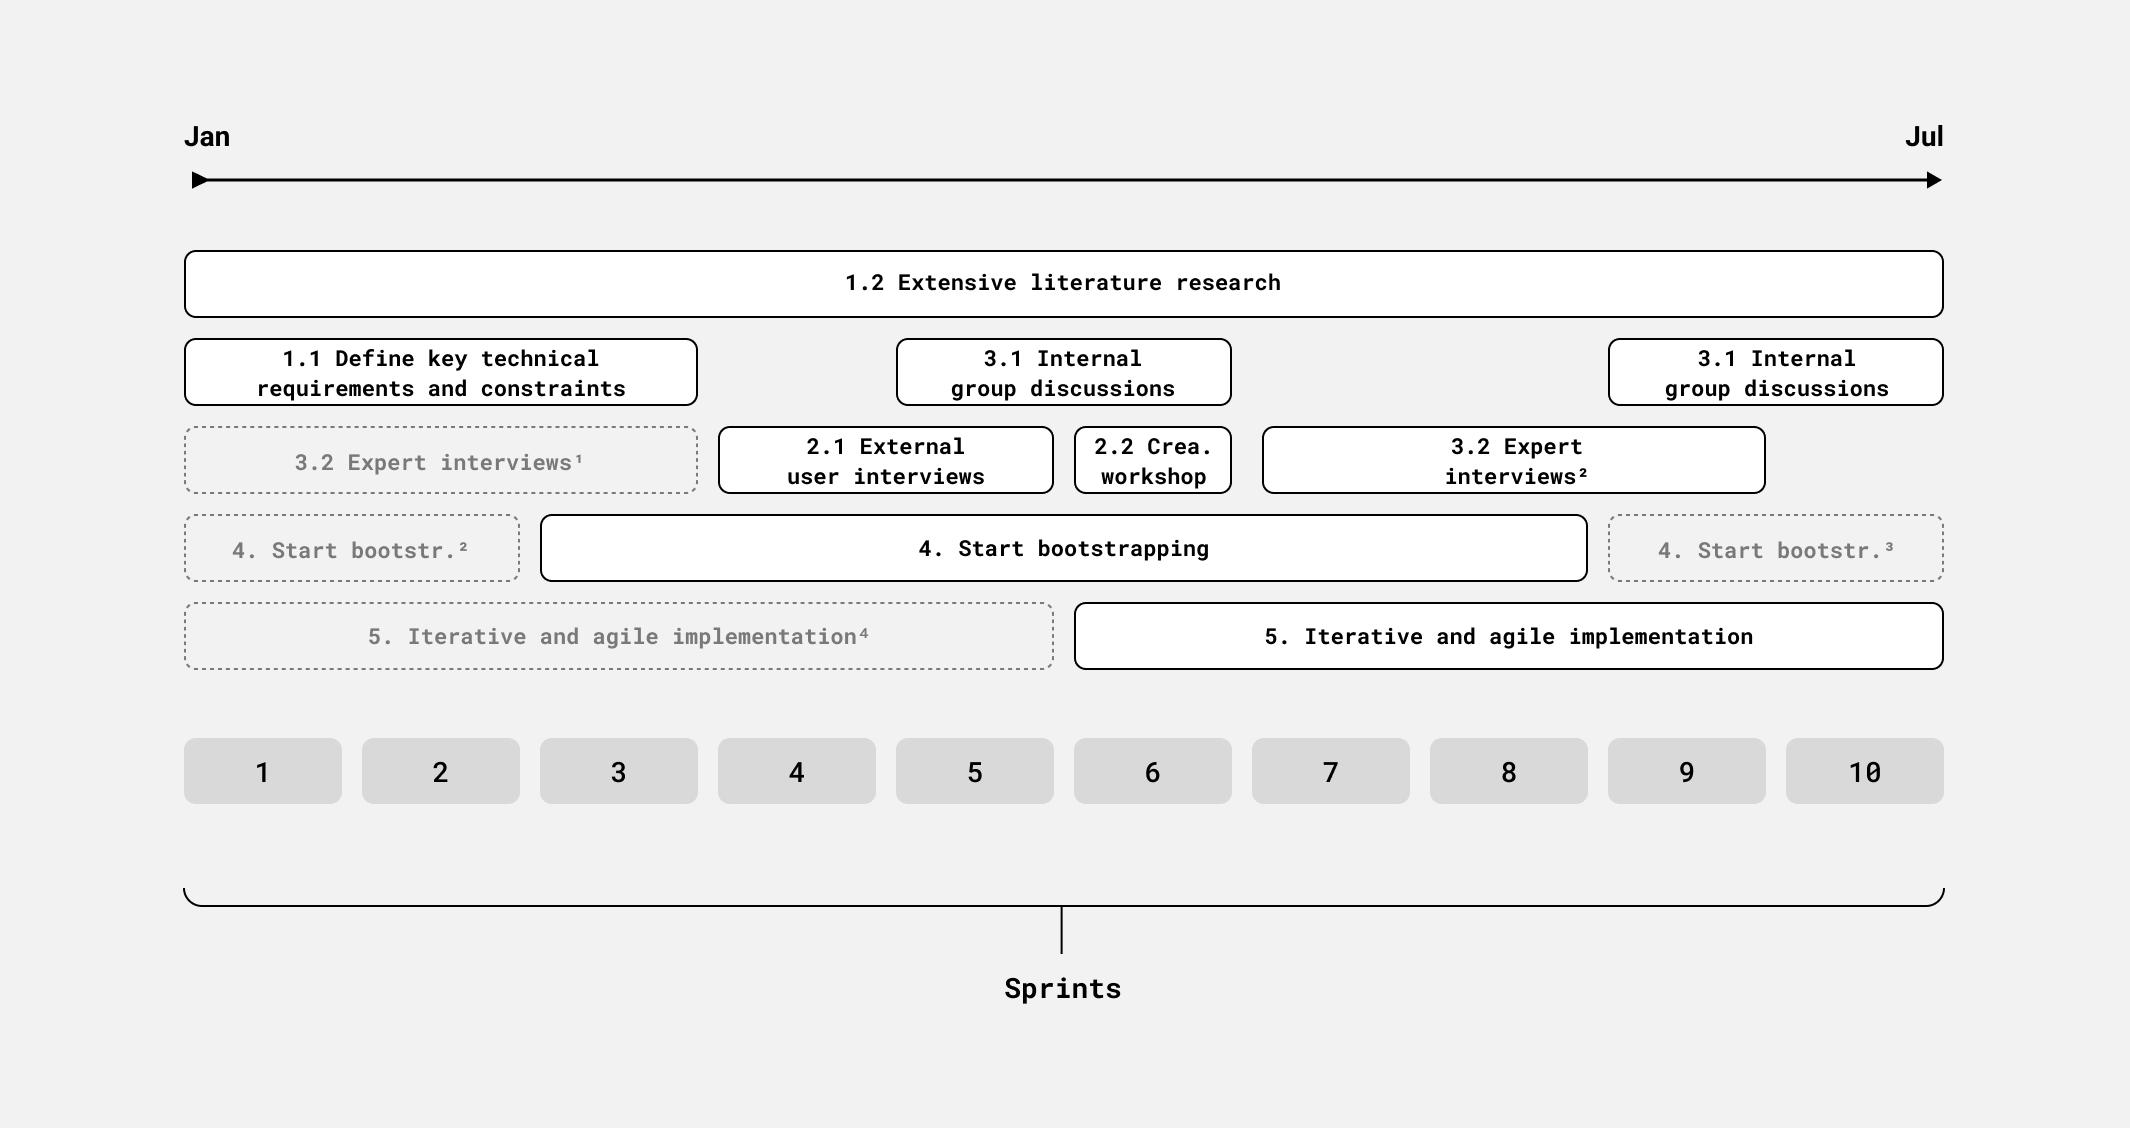
\includegraphics[width=\linewidth]{implementation-timeline.png}
  \caption{Effective timeline of the last ten sprints with project stages in white and specifically planned stages outlined in grey.}
  \label{fig:implementation-timeline}
\end{figure}

\begin{table}[ht]
\centering
\resizebox{\textwidth}{!}{%
\begin{tabular}{
>{\columncolor[HTML]{FFFFFF}}l l}
\cellcolor[HTML]{000000}{\color[HTML]{FFFFFF} Special stage} &
  \cellcolor[HTML]{000000}{\color[HTML]{FFFFFF} Description} \\ \hline
\multicolumn{1}{|l|}{\cellcolor[HTML]{FFFFFF}\textbf{\begin{tabular}[c]{@{}l@{}}[1] 3.2 Expert\\ interviews\end{tabular}}} &
  \multicolumn{1}{l|}{\begin{tabular}[c]{@{}l@{}}The author was able to use the first expert discussions in advance thanks to the help of one\\ of the sales staff's networks. The experts were Nuvibit's experienced enterprise cloud and\\ solution architects. The first topics were strictly technical in nature, focusing on medium-\\ term technological decisions in the context of the company and the timetable.\end{tabular}} \\ \hline
\multicolumn{1}{|l|}{\cellcolor[HTML]{FFFFFF}\textbf{\begin{tabular}[c]{@{}l@{}}[2] 4. Start\\ bootstrapping\end{tabular}}} &
  \multicolumn{1}{l|}{\begin{tabular}[c]{@{}l@{}}This special stage describes the phase in which the author established more organisational\\ structures, such as a professional Scrum or GitHub setup. Furthermore, the time was used\\ to create a more professional AWS organisational setup with various organisational units,\\ as described in the AWS Best Practice Guide \citep{blackham_best_2020}.\end{tabular}} \\ \hline
\multicolumn{1}{|l|}{\cellcolor[HTML]{FFFFFF}\textbf{\begin{tabular}[c]{@{}l@{}}[3] 4. Start\\ bootstrapping\end{tabular}}} &
  \multicolumn{1}{l|}{\begin{tabular}[c]{@{}l@{}}Since the creation of two different Python SDKs (as discussed later in the thesis), more\\ bootstrapping tasks were due at the very end of the given time frame, mostly including\\ the setup of a private PyPi installable Python package and SDK-specific quality\\ assurance pipelines and automations.\end{tabular}} \\ \hline
\multicolumn{1}{|l|}{\cellcolor[HTML]{FFFFFF}\textbf{\begin{tabular}[c]{@{}l@{}}[4] 5. Iterative and\\ agile implementation\end{tabular}}} &
  \multicolumn{1}{l|}{\begin{tabular}[c]{@{}l@{}}Iterative and agile implementation began as soon as needed, without waiting for the design\\ process to be completed (i.e. avoiding a waterfall process). Prior to gaining insights from the \\ design process, time was spent on everything else, such as evaluating technologies, further\\ bootstrapping, first example codebases, or maintaining the old codebase a bit.\end{tabular}} \\ \hline
\end{tabular}%
}
\vspace{10pt}
\caption{Special project stages in the effective schedule as shown in \autoref{fig:implementation-timeline} and their explanation of why they took place there.}
\vspace{-5pt}
\label{tab:special-project-stages}
\end{table}

Several key events occurred during the implementation that shaped the future course of the project and research. This was primarily due to initially unplanned early expert discussions or uncertainties in the requirements as the user-centred design process was still being prepared. These key events are overlaid with the effective project plan as shown in \autoref{fig:implementation-timeline-key-events}. These three green key events are the most influential key events.

\begin{figure}[!ht]
  \centering
  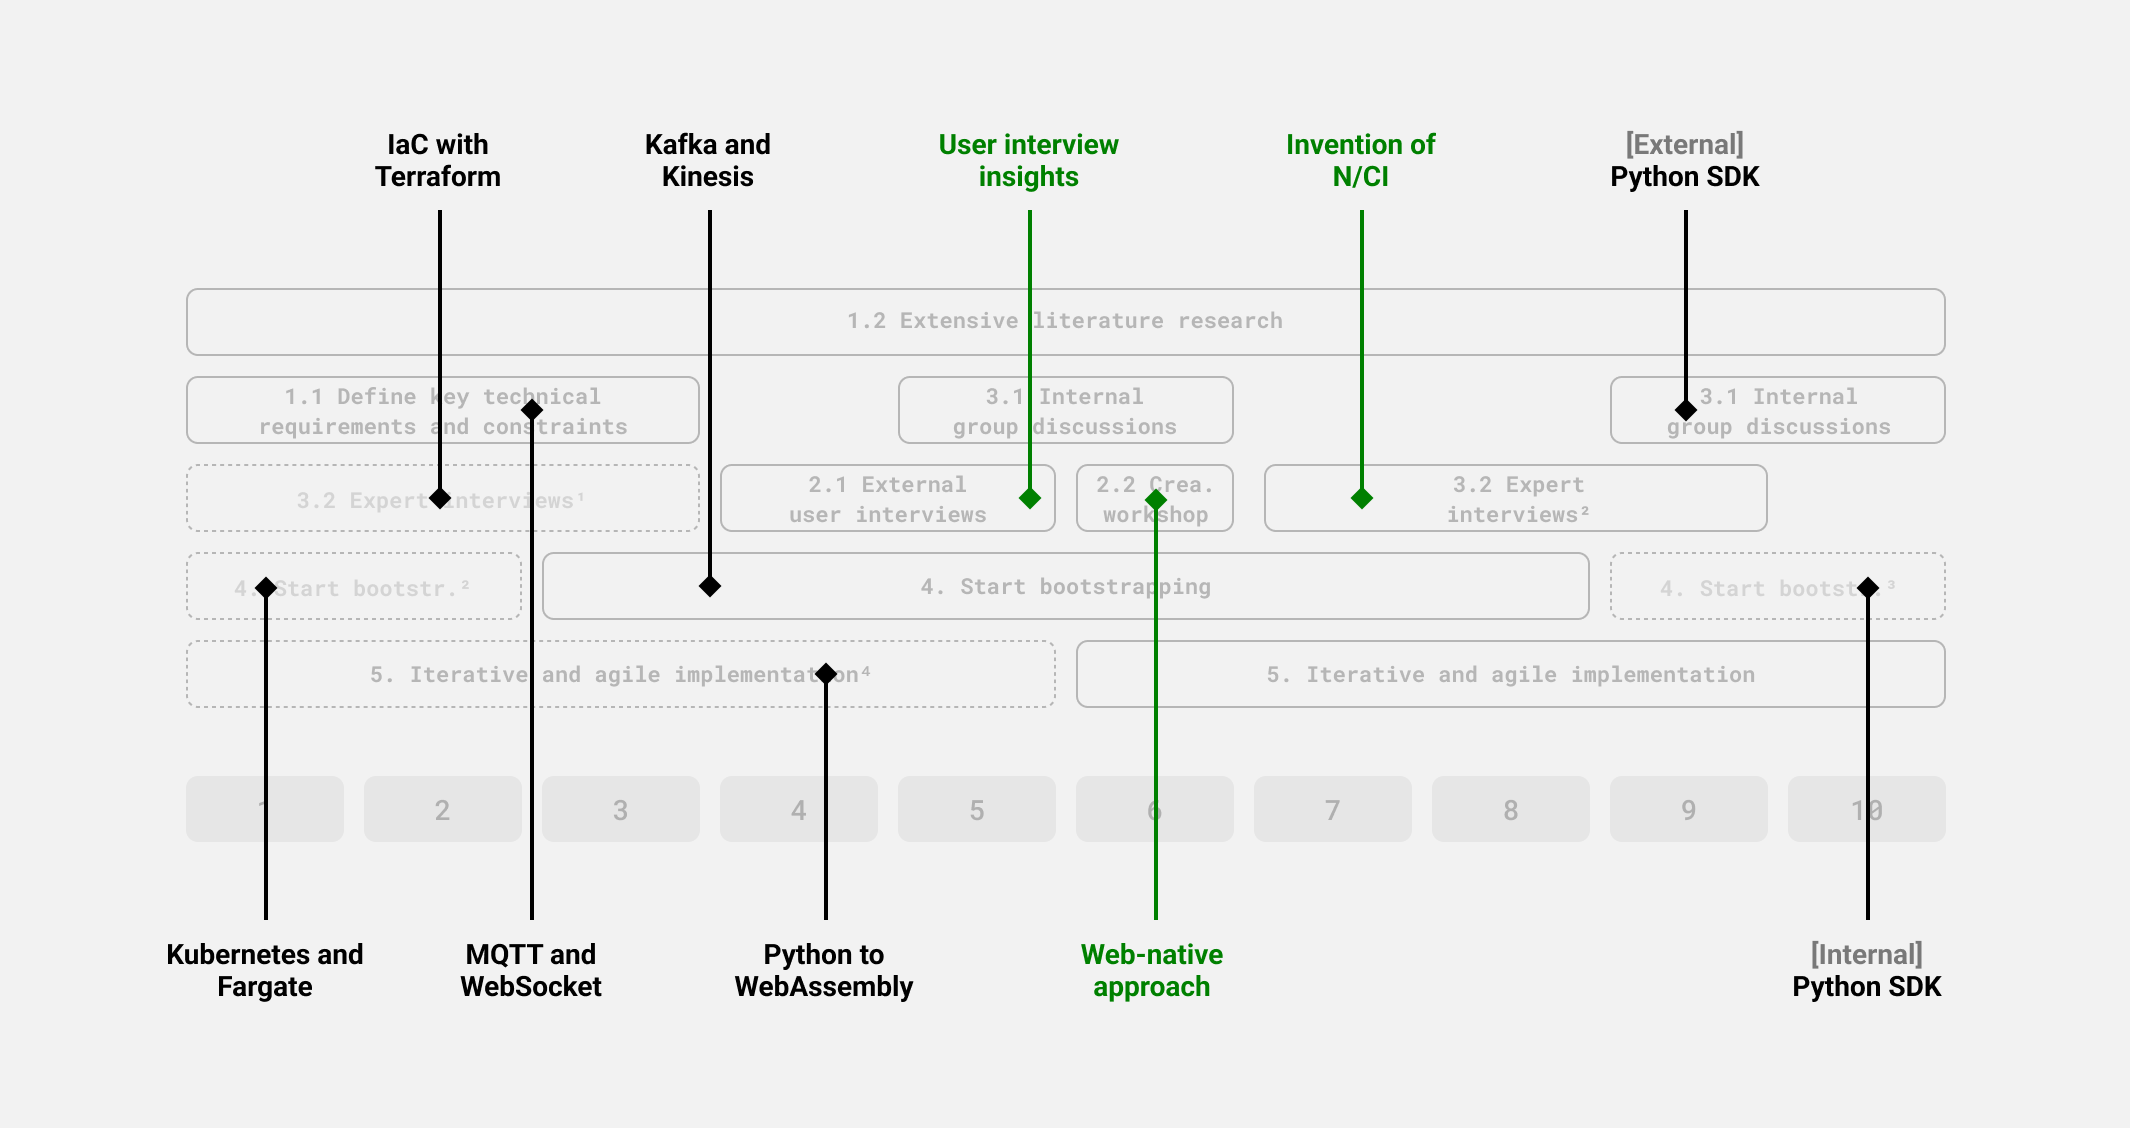
\includegraphics[width=\linewidth]{implementation-timeline-key-events.png}
  \caption{The key events overlaid on the effective project schedule as illustrated in \autoref{fig:implementation-timeline}, with the most influential events coloured green.}
  \label{fig:implementation-timeline-key-events}
\end{figure}

% empirical software engineering done in the case study based on a user-centred design process via user interviews, expert interviews, internal group discussions, and ongoing literature research.
% MENTION analysis paralysis

\section{Key events while building a N/CI}
\label{chapter4-key-events}

This section goes over each key event as shown in \autoref{fig:implementation-timeline-key-events} and discusses why it happened and was critical to the project's success. The following outline of the key events is not chronologically described but instead starts with the most influential ones.

\subsection{User interview insights}
\label{chapter4-user-interview-insights}

The conduct of user interviews was one of the most influential key events. This process began with the development of customer personas based on the sales team's previous experiences with real customers and the planned customer segments targeted by C-level management. The author does not want to go into too much detail about how the personas were created and how the process went, because the focus is on the results based on the user interviews, not on the persona creation process itself. The personas are illustrated in \autoref{fig:personas}, and a more detailed version is included in \autoref{appendix4-screenshots}.

\begin{figure}[!ht]
  \centering
  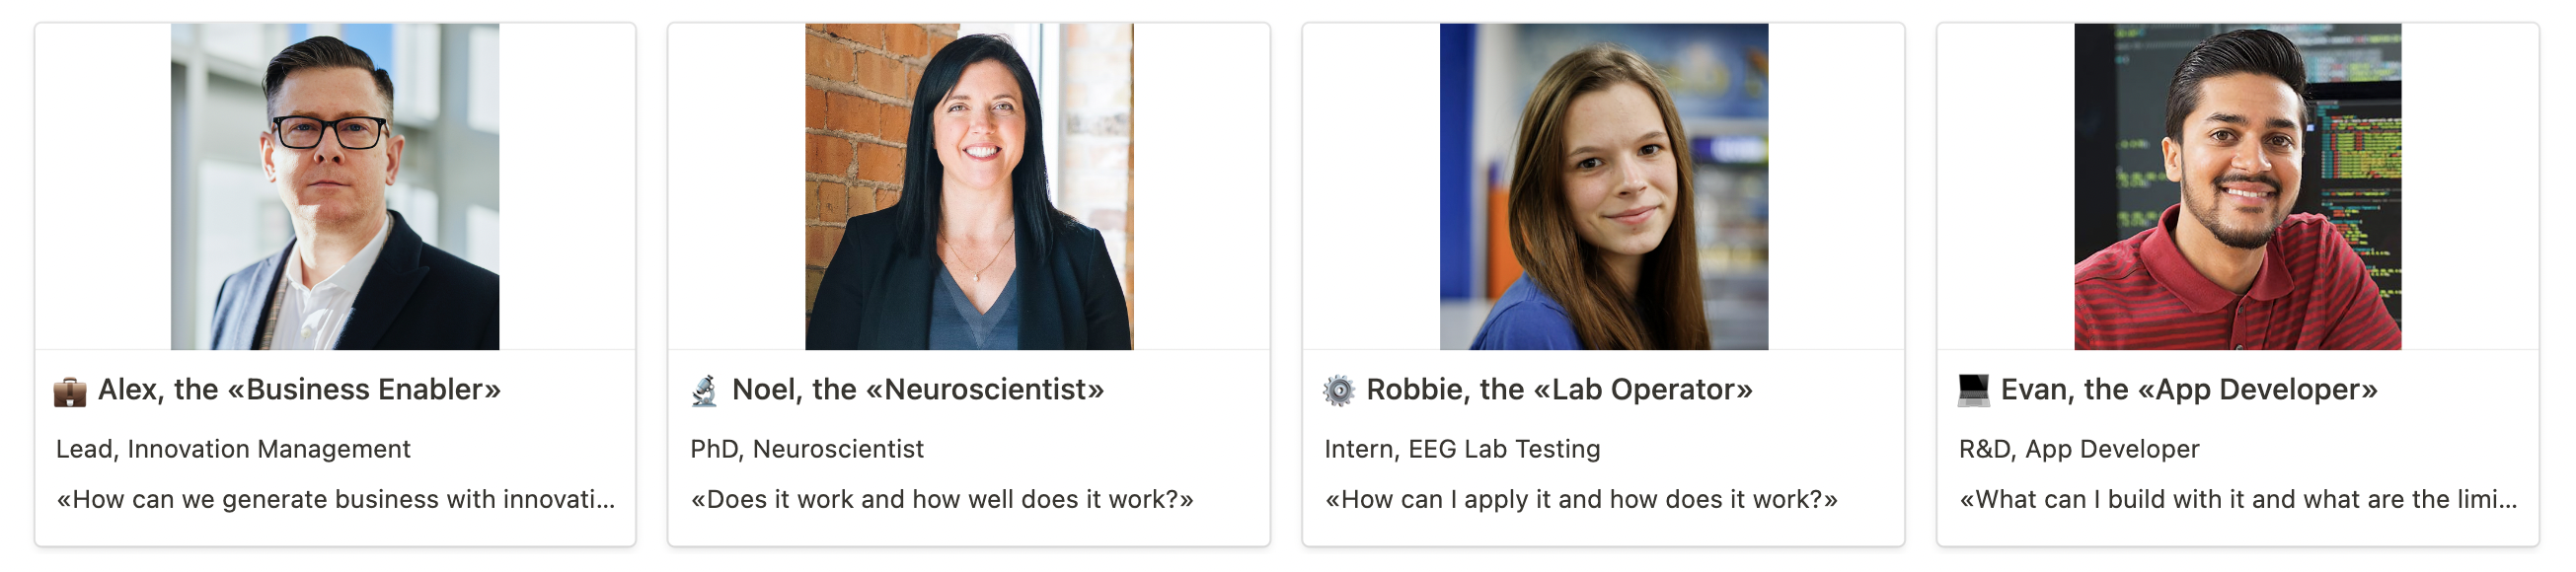
\includegraphics[width=\linewidth]{personas.png}
  \caption{IDUN's customer personas.}
  \label{fig:personas}
\end{figure}

Real people were then chosen to represent the personas as accurately as possible. The IDUN staff scoured their network to accomplish this. Finally, the author compiled a list of twenty individuals. Seven people were chosen from this list and invited for separate interviews. The interview outline was planned in collaboration with IDUN's product manager and an industry UX expert, Laura Bendixen, who works as a UX designer at Blick.ch. The author completed the outline based on Laura's expertise with previously conducted user interview sessions, which can be found in \autoref{appendix1-user-interviews}. All user interviews were conducted remotely and lasted no more than 1.5 hours. During the interviews, insights were transcribed on post-its. People working with BCIs or EEG were interviewed, as were PhD students working in research labs, developers who e.g. had never worked with BCIs or had extensive experience building even own BCI software, and business-enablers from companies responsible e.g. for BCI-based accessibility. More details about the chosen individual interviewees can be found in \autoref{appendix1-user-interviews}.

The questions were non-leading open-ended, with the main goal of allowing interviewees to express themselves and capturing their perceptions of the BCI industry and upfront introduced IDUN vision and mission. The goal was to determine what software offerings a mass-market BCI-software device would need to provide, such as convincing developers who have never worked with BCI to include neuro-enhanced features, or convincing researchers to use IDUN's NIP in their research. The questions and answers were all about different things. More technically oriented people inquired about speed, performance, and privacy concerns (ergo more production-readiness thinking), whereas researchers inquired about signal quality, the ability to synchronise with other data streams, and access to raw data (more general applicability thinking). After the last user-interview, all post-its were compiled, similar insights were grouped and the product manager as well as the author categorised the most important insights into a list:

\begin{itemize}
  \item \textbf{There are two prominent use cases: using the NIP for research and developing an end-user-facing app.} These are two critical distinctions. Researchers would use the NIP to learn about the brain due to data that was previously cumbersome to collect, such as through simple-setup remote experiments or real-life long-term experiments outside of laboratories. The NIP would, in such a use case, still be used in production, but not to potentially thousands or millions of users in an app intended for end users. The company or developer using the NIP would have physical access to the hardware in the research use case, because they would most likely buy one or more devices and hold them in their reservoir. In contrast, companies targeting production use cases would ship the devices as, e.g. white-labelled hardware through their own or 3rd-party channels. Perhaps we can even go so far as to say that because IDUN distributes the device so well, companies and developers do not need to sell the device themselves but can simply assume that users own such headphones and then access the brain API such as e.g. today's developers can just assume that every end-user has GPS access in their smartphone.
  \item \textbf{Visual demos that are easily accessible for someone owning the hardware are important for all personas, most importantly an Alex.} A visual and simple demo should demonstrate what one can do with the NIP from IDUN and inspire others to conduct research, build apps or enable business and opportunities. These demos need to explain to the different personas the different benefits; next to that also, the end-user should be able to try out the demos to see the benefits of BCI-enhanced technologies. People such as Evan should be able to adapt demos with their own codes to, e.g. create their own version of them.
  \item \textbf{The user of the NIP needs to have as low-level control over the data flow and classification as possible} but also with an option for less technical users to use it and build things, similar to e.g. AWS: AWS itself is only an API to use cloud IT resources, but they also have the AWS Console app to build everything via a GUI instead only via the API. What is very important here is that people such as, e.g. Noels need to know exactly what algorithms were used or what the methodologies for certain classifiers are in order to justify them and integrate them into their research. They do not, in most instances, actually need raw data access, as plotting functionality would also be enough; therefore, IDUN's NIP should have somewhere functionalities to plot and visualise data.
  \item \textbf{In order to ease the use of the GUI and the API of the NIP, IDUN needs to provide, next to satisfying documentation, libraries for certain environments} that make the unobtrusive implementation of the NIP easier. Such as, e.g. providing a client-side JavaScript package that is lean and easy to use that can be integrated simply into existing apps. Examples for such code integration would also need to be provided by IDUN so that people like Evan can easily adjust them and more quickly start integrating them into their apps or research codebases. The personas would need to be able to abstract the brand IDUN as much as possible away as, e.g. Intel is doing with their Intel-inside ingredient strategy \citep{intel_ingredient_nodate}.
  \item \textbf{End-users need control over their data so that other companies accessing the NIP API cannot collect their data} on their servers and do everything what they want with it. Imagine if e.g. the operating system layer of ones smartphone would not offer an opt-in mechanism for the cameras, then 3rd-party developers could just install spyware and record without the user giving permission for it. When e.g. users start to use multiple apps with a NIP integration, there needs to be some way to control the opt-in and data access without the app developers having any saying on the decisions. There needs to be a technical limitation from the side of the hardware or the cloud to ensure user privacy and data security for end-users.
  \item \textbf{Researchers are very interested in the raw EEG data and the synchronisation possibilities with certain protocols} such as LSL to combine, e.g. a heart rate sensor with the EEG collected from IDUN's hardware. The NIP software offering need to give enough freedom to combine the data without letting all other collected data flow into the NIP from IDUN. This basically means that the NIP should be able to collect, transform and, most importantly, label data in correlation with other data streams with a local option to satisfy researchers like Noel.
\end{itemize}

These insights were critical in determining that there must be sufficient freedom for raw data research without releasing raw data into mass market production environments in order to protect end-user privacy. As a result, an opt-in mechanism outside of third-party ecosystems is required. A library that can be implemented in end-user apps and connects directly to the hardware without the need to download a companion app from IDUN itself is also required. This library should allow researchers to access it locally and, e.g. use their preferred protocols to synchronise tags and labels with other data streams. Nonetheless, IDUN's NIP should once again provide some control over how much raw data can be collected and restrict access if, e.g. the proposed research project or experiment time frame is exceeded. Furthermore, additional NIP functions should be added to visualise easy-to-use demos for all personas, as well as a way to use and control the NIP without having to write code, but with enough flexibility and transparency that there is trust in the system and even advanced users can work with a visual tool instead of code.

\subsection{Invention of N/CI}
\label{chapter4-invention-of-nci}

The insights from the user interviews, combined with the ongoing research on B/CI and remote BCI mentioned in the introduction chapter, were key to realising the novelty of this new interdisciplinary approach to developing a real-world and mass-market BCI software system running in the cloud and targeting the general population via general applicability. In this thesis, the definition of three-dimensionality was already mentioned in the context chapter, but it is important to mention that the realisation that such a system is novel and has not yet been defined only emerged in the seventh sprint. The findings from the user interviews were primarily in the direction of the N/CI definition, while the literature review was primarily in the direction of distinguishing between existing research and definitions.

Once a first draft of the definition was written down, the research and separation of work packages could be more easily tackled and explored due to a better understanding of what was new and unexplored. At the time of the end of the seventh sprint, the author's goal was to further develop and define the definition and motivation in the form of the last part of the context chapter of this thesis, which had to be introduced first before moving on to the methodology and implementation chapters, because without a broad understanding, the reasons for the motivation and the general definition would have been difficult to understand.

\subsection{Web-native approach}
\label{chapter4-web-first-approach}

Before Sprint 6, there were some ideas about future architecture roadmaps designed by the author of this thesis, as shown on \autoref{fig:architecture-roadmap}.

\begin{figure}[!ht]
  \centering
  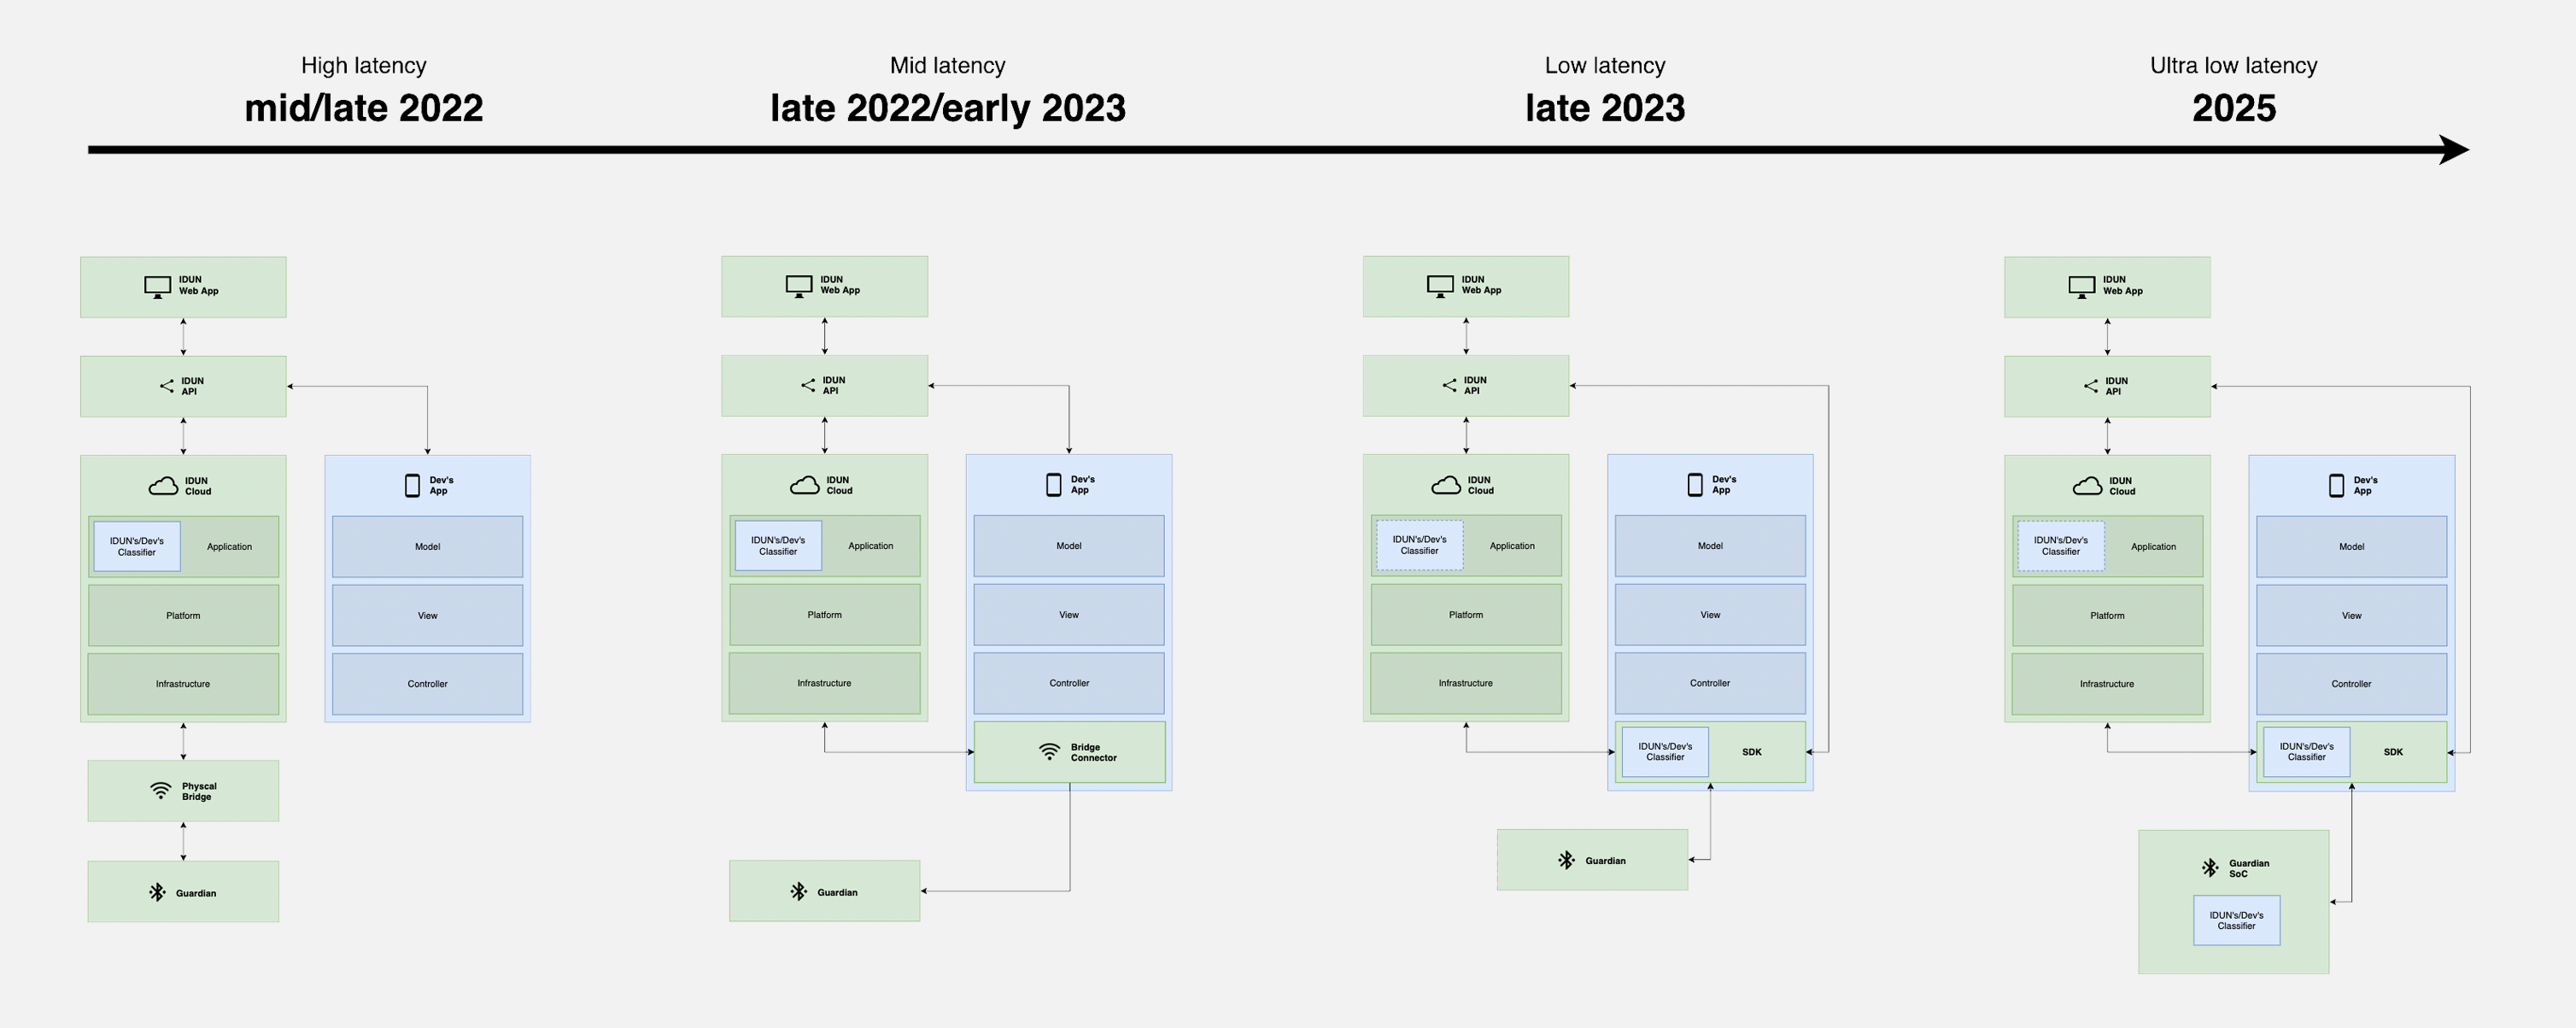
\includegraphics[width=\linewidth]{architecture-roadmap.png}
  \caption{Original architecture roadmap of IDUN's NIP.}
  \label{fig:architecture-roadmap}
\end{figure}

The initial architecture roadmap was part of the initial phase of the project to define the key technical requirements and constraints and to show how the NIP software stack would move from a high latency system to an extremely low latency system. More details on the latency aspects are discussed later in this chapter. Nonetheless, one aspect of this old architecture roadmap was that IDUN would continue to maintain and develop the physical hardware network bridge and eventually port it to end-user devices as a companion app. However, just before Sprint 6, the author stumbled upon the work of \citeauthor{flynn_brainsplay_nodate} of the BCI platform called Brains at Play and its use of Web Bluetooth, which is a new and experimental API for browsers that allows websites to connect directly to a Bluetooth Low Energy (BLE) device. The Brains at Play platform is a hardware-independent BCI software platform with similar goals to Neuromore Studio. The main difference is that they offer their app as a web app and therefore everything runs in the browser without the need to download additional software. The author contacted Garrett Flynn, one of the founding partners, and discussed the implications and findings from using Web Bluetooth for e.g. EEG data such as that from IDUN's sensor (later Garrett Flynn was also invited to the user interviews as one of the persona representatives for Evan). Garrett Flynn's findings were entirely positive and he strongly recommended working with the API as it makes deploying a BCI platform much easier than deploying applications for any operating system and especially any BLE interface. However, one of the main disadvantages of Web Bluetooth was browser compatibility, as shown in \autoref{fig:can-i-use}.

\begin{figure}[!ht]
  \centering
  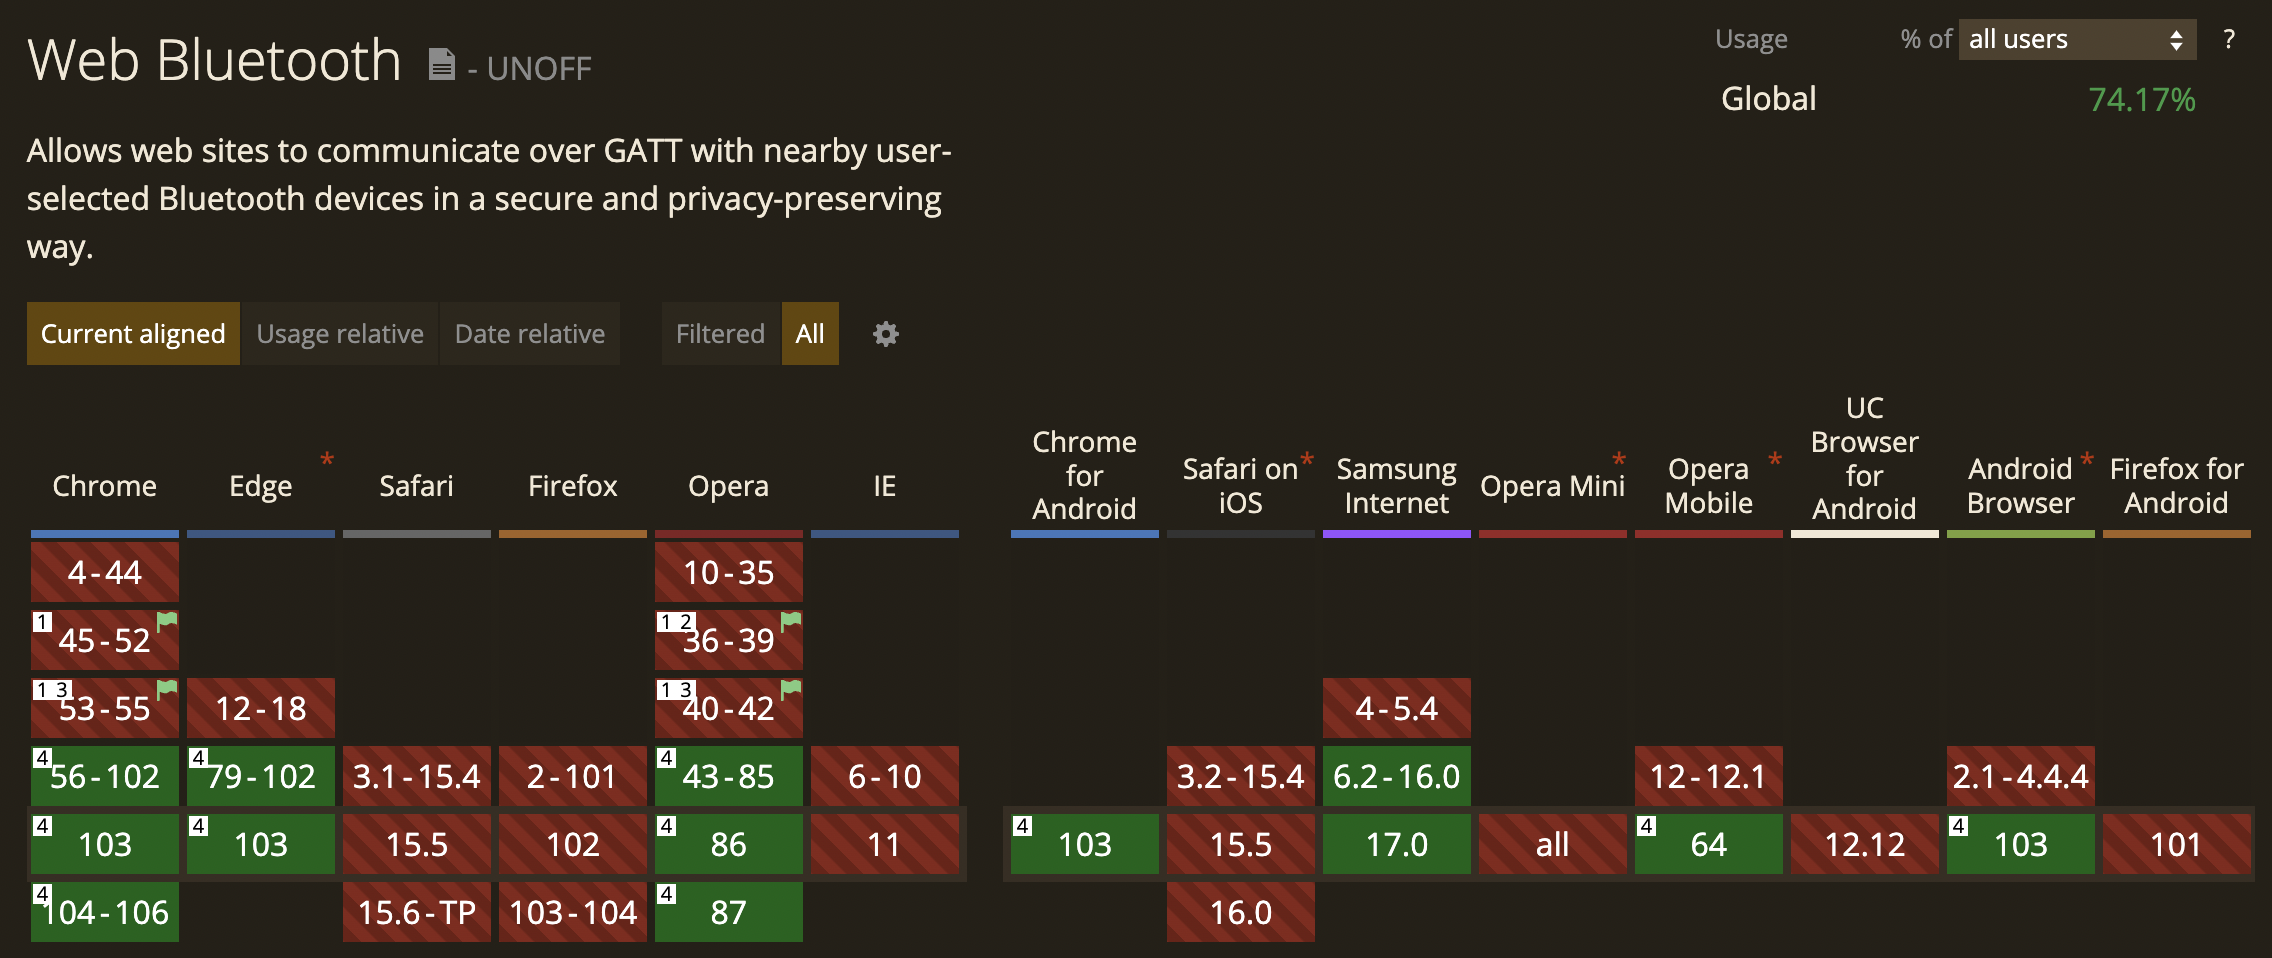
\includegraphics[width=\linewidth]{can-i-use.png}
  \caption{Browser compatibility overview of Web Bluetooth \citep{caniuse_web_nodate}.}
  \label{fig:can-i-use}
\end{figure}

Nevertheless, IDUN is building a product that aims for the big future in 2-3 years, as can be seen on their roadmap in \autoref{fig:idun-timeline}, which means that browser compatibility could come and ease-out over the coming years once browser manufacturers start implementing the API. One problem, however, is that the web Bluetooth API cannot be run in a service worker, making it impossible to run in the background when, e.g. the device has its screen locked or another app is currently opened on a smartphone \citep{webbluetoothcg_service_2018}, which is an intermediate problem, even for the upcoming smaller and specific user groups with the current personas. While researching Web Components, the author came across another technology: Capacitor, a JavaScript library that can compile and run web apps as native apps, with the ability to access native APIs \citep{ionic_capacitor_nodate}, such as the camera or, especially important for IDUN, the BLE API \citep{capacitor-community_capacitor-communitybluetooth-_2022}. Developers can use Capacitor to write BLE code with the same interface as Web Bluetooth, compile the code and run the applications on native devices with background functionality.

After further research, as shown in \autoref{appendix4-screenshots}, almost the entire Sprint 6 was spent evaluating the possibility of using Web Bluetooth for IDUN's NIP. At the end of the sprint, a working PoC SPA was created with an iOS and Android build that fulfilled all needs in terms of developer experience, latency of the EEG signal from the device to a visualisation plot and power consumption of lower-end smartphones. Following this, the author proposed to change the original architecture roadmap as depicted on \autoref{fig:architecture-roadmap} and skip the first two steps and go directly to step 3 in order to accelerate the development pace and enable greater market maturity for IDUN's NIP as soon as end of 2022.

The use of a web app, combined with the use of modern APIs and the compilation of the app for mobile applications when compatibility is not guaranteed is called a web-native approach \citep{ionic_web_nodate}. Besides the time saved by not having to develop platform-specific apps but using a single code base, this approach also has the advantage that a library that abstracts the logic of connecting a BLE device such as the IDUN device can already be created into a single installable unit, e.g. in the form of an NPM package. This library can be implemented in end-user apps and connects directly to the hardware without the need to download a companion app from IDUN itself, and is one of the solutions to the findings from the user interviews. The time saved with a web-native approach allowed IDNU to already focus on creating such a library and using it in their own web app, which would be the console or GUI as in the AWS example, allowing dogfooding for our own software offerings and eliminating preliminary issues before releasing the library to the public \citep{techopedia_what_2016}.

\subsection{Python to WebAssembly}
\label{chapter4-python-to-webassembly}

Another key event that happened during the ten sprints took place about two sprints before the evaluation of the web-native approach. The idea was that, as mentioned in \autoref{chapter3-software-and-tools}, when it comes to how important and necessary the Python ecosystem is for IDUN and external people as presented in the personas, it might be possible to create Python code for specific neural signal data processing, compile it to WebAssembly, a low-byte compilation target for high-level languages that run mainly in the browser, and then use it in web applications such as e.g. the GUI application of IDUN's NIP. Sprint 5 evaluated compiling Python into WebAssembly, which seemed promising at first, but then turned out to be too far away from today's possibilities. There is an interesting open source project called RustPython, which is an Python interpreter written in Rust that allows the interpreted code to be compiled in WebAssembly. However the maturity of the project is currently not suitable for production, as it is even mentioned by the maintainers themselves \citep{noauthor_rustpython_2022}.

Another option would be to use Pyodide, the CPython interpreter ported to WebAssembly \citep{noauthor_pyodide_2022}. Apart from the fact that the creation of a web application would be drastically larger if a complete Python interpreter were sent to the browser, this interpreter also does currently not have the functionality to add additional Python packages apart from the standard library from e.g. PyPi, which makes it easy to build vanilla Python on top of WebAssembly codebases, but not with custom packages installed, such as machine learning packages needed for EEG classifiers. The only options left were to develop an own Python to WebAssembly compiler, contribute to the two open source projects, or give up the task of embedding Python code in a web application such as IDUN's GUI application to interact with NIP's API. The latter was chosen because it was still too early, immature and time-consuming, as the results of Sprint 5 showed.

\subsection{Kubernetes and Fargate}
\label{chapter4-kubernetes-and-aws-fargate}

One of the first technical decisions the author of this thesis made was which technology to use for creating backends for an n-tier\footnote{The term n-tier refers to an architecture design pattern where the logic of presentation, application processing, and data management are decoupled from each other, as in the case of e.g. multiple microservices.} system like IDUN's NIP. The use of a microservice approach was already given by the fact that a polyglot backend was needed, such as Python for data-heavy tasks and TypeScript for real-time and API-specific tasks due to the maturity in the previously mentioned examples of each language. If one decides to take a microservice approach, one can still debate whether to proceed with serverless functions instead of hosting container images. Given the requirement to use AWS mentioned in \autoref{chapter3-software-and-tools}, the only way to host serverless functions was to use AWS Lambda. AWS Lambda was already used in the previous PoC version of the software system at IDUN and did not work as well as in cases where, for example, batch processing of previously collected data would exceed the maximum computation time or CPU limit of AWS Lambda. This, coupled with the cumbersome aspect of handling dozens if not hundreds of serverless functions and managing the entire "cluster" of multiple functions and their versions and endpoints, led to the decision not to use Lambda for the most important and critical parts of the backend in the author's experience so far.

Building microservices not with serverless functions on AWS has multiple solutions: the most prominent ones are utilising Kubernetes via AWS Elastic Kubernetes Service (EKS) or AWS Fargate, which is a serverless and easier-to-use version of Kubernetes \citep{aws_serverless_nodate}. The author consulted cloud experts in the very first sprints from the company Nuvibit to guide through the decision. The author himself is not experienced in Kubernetes and would need to learn a lot of things on the way to implement a Kubernetes cluster which was one of the items mentioned to possibly avoid mentioned in \autoref{chapter3-software-and-tools}. Nuvibit recommended going with AWS Fargate, since it is similar to Kubernetes but abstracts most things away in order to concentrate on adding business logic rather than handling overheads coming with introducing a Kubernetes cluster. Fargate is per-se also serverless, therefore making it cheaper for a product with hard-to-estimate usage such as IDUN's NIP in the beginning but still gives enough flexibility in terms of specifying the underlying hardware for computationally heavier tasks that e.g. would exceed AWS Lambda. As soon as IDUN goes more into the direction of utilising large-scale deep learning models that utilise specific GPU units, Fargate will come to its limits since specifying GPU tasks is not possible \citep{aws_aws_2019}. One way or another, this decision will have to be reconsidered in the future in order to avoid a long-term commitment to one provider such as AWS and to due to the increasing investments of Kubernetes from several cloud providers.

\subsection{Kafka and Kinesis}
\label{chapter4-kafka-aws-kinesis}

Another early technical decision, made with the help of expert interviews, was which streaming technology to use. As with many things in software, there are hundreds, if not thousands, of ways to solve a problem such as streaming text-based data like the EEG data from IDUN's device over the internet to the cloud. Apache Kafka, originally developed by LinkedIn, is a very prominent technology for such a use case. It is battle-tested, used in production by large technology companies \citep{apache_apache_nodate} and well maintained by an active community \citep{noauthor_apache_2022}. However, similar to Kubernetes, it comes with a lot of overhead, and the author himself has no experience with Kafka, so again he would have to learn everything from scratch. Another option is to use AWS Kinesis, a service provided by AWS to process data streams over the cloud, like Kafka does, but without the overhead of managing the Kafka instances themselves. AWS Kinesis allows streams to be replayed, restored, sent to an AWS Fargate cluster for e.g. real-time processing of the data, or data to be stored securely in storage systems such as AWS Simple Storage Service (S3), as shown on \autoref{fig:aws-kinesis}. An important aspect is that the source of the data can also come from a WebSocket stream, which will be addressed in the next section. However, the decision for Kinesis was quite easy, as the reasoning was similar to that between Kubernetes and AWS Fargate. The decision was also supported by the experience and opinion of the cloud experts at Nuvibit.

\begin{figure}[!ht]
  \centering
  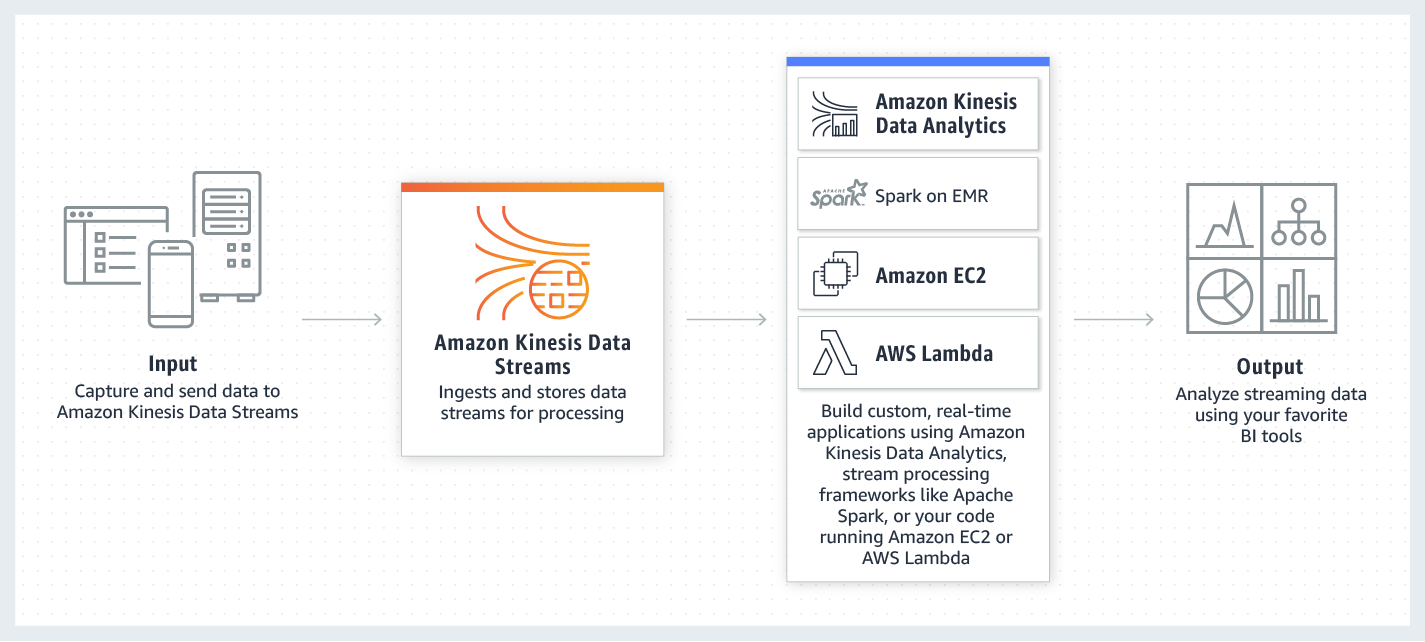
\includegraphics[width=\linewidth]{aws-kinesis.png}
  \caption{Example use-case architecture of AWS Kinesis \citep{aws_amazon_nodate}.}
  \label{fig:aws-kinesis}
\end{figure}

\subsection{MQTT and WebSocket}
\label{chapter4-mqtt-and-websocket}

As previously stated, a decision had to be made regarding the technology to be used to transfer data from a physical device, such as IDUN's EEG sensor hardware, to the cloud. Previous engineers at IDUN used MQTT to stream data from the hardware directly to the web app, as mentioned in the list of bugs and flaws in \autoref{chapter3-derivation-of-the-case-study}. MQTT is not well suited to sending high-frequency data in real time, such as EEG, and it is geared toward lower-power IoT devices rather than, say, a computer or smartphone to which the IDUN device would be connected. As a result, the decision to use something else had to be considered. Another option is to use WebSocket, which is designed for high-frequency updates that can be updated in real time in both directions. The reason IDUN would want to use a high-frequency protocol is that e.g. HTTP can only handle about ten requests per second, whereas e.g. WebSocket can handle nearly 4000 requests in the same amount of time. The main reason for this significant difference is that e.g. the browser limits the number of concurrent HTTP connections, whereas a WebSocket connection has no limit on the number of messages it can send or receive \citep{luecke_http_2018}. Sending EEG data at a frequency rate of 250 samples per second from the IDUN hardware and receiving multiple classification responses from the cloud based on the chosen classification certainly necessitates more than ten requests per second.

\begin{figure}[!ht]
  \centering
  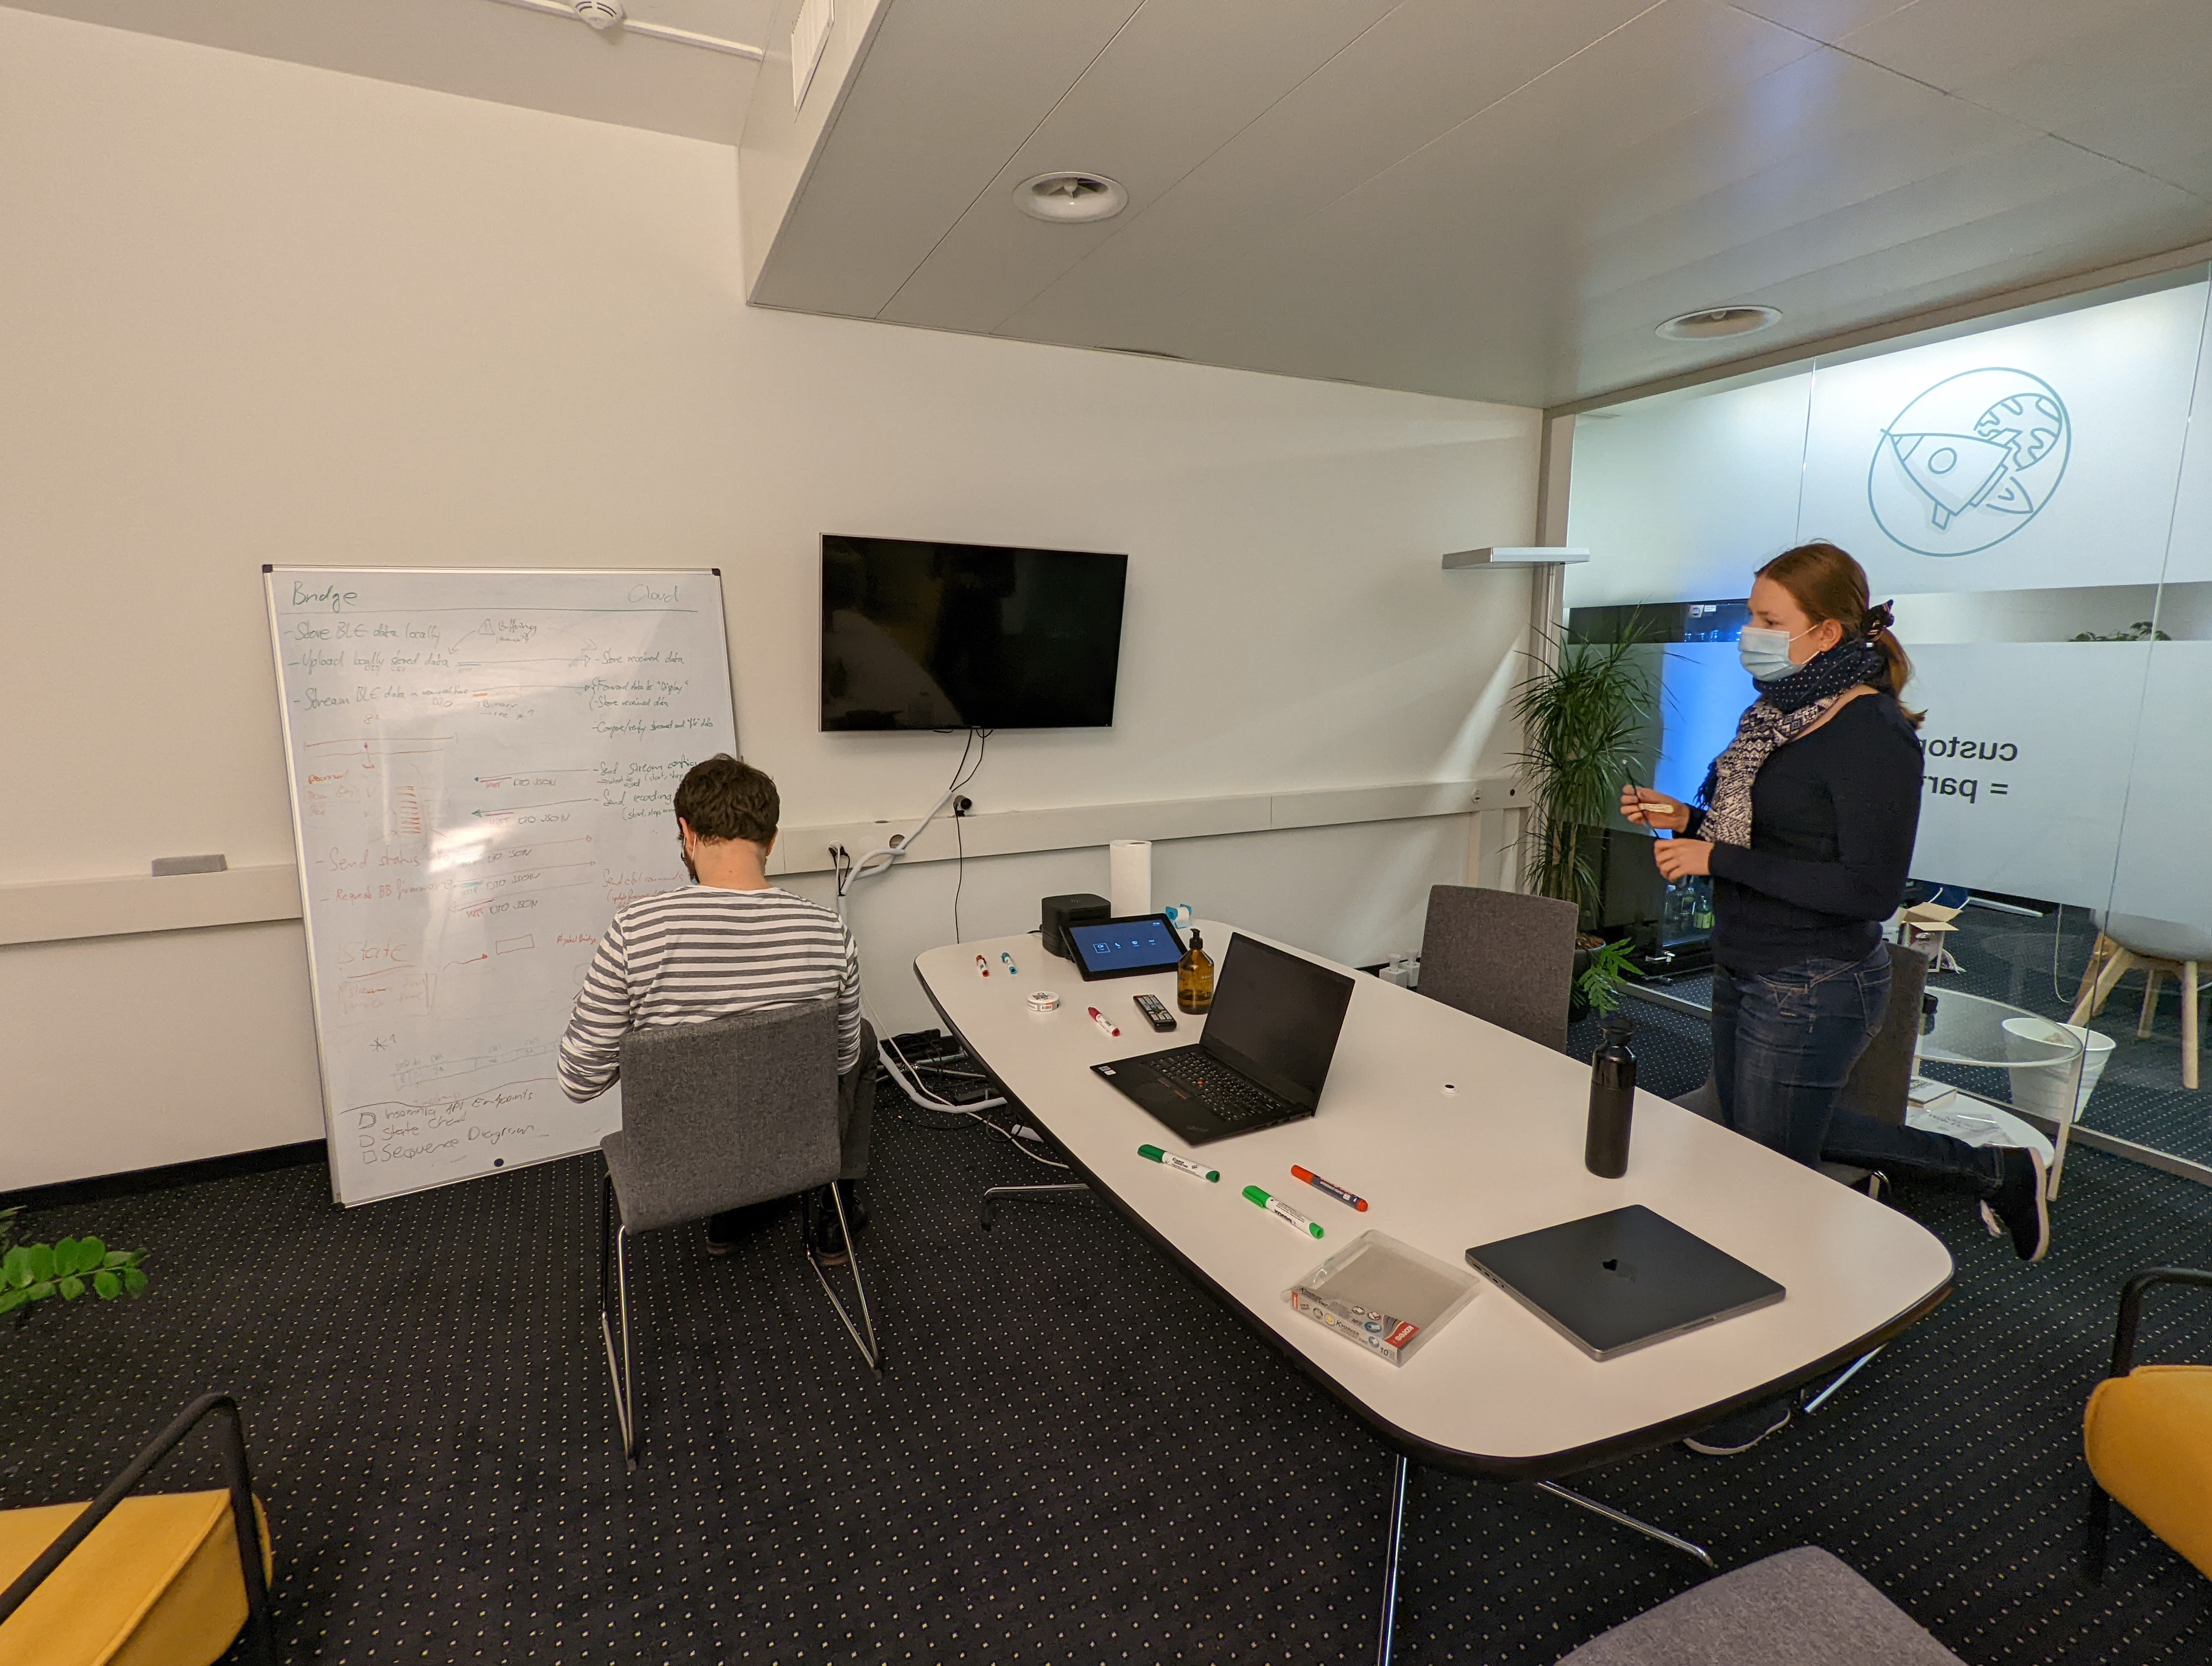
\includegraphics[width=0.75\linewidth]{firmware-engineers.jpeg}
  \caption{Photo of an internal group discussion with the firmware engineers from IDUN.}
  \label{fig:firmware-engineers}
\end{figure}

WebSocket also integrates easily with the earlier technology decision for AWS Kinesis, as Kinsesis can subscribe to an API gateway service from AWS that can be used to build Representational State Transfer (REST) APIs (more on this in \autoref{chapter5-main-results}). An internal group discussion with firmware engineers for IDUN's hardware was organised to validate this decision as shown on \autoref{fig:firmware-engineers}, as it was too BCI specific to ask e.g. Nuvibit's cloud engineers. The alignment with the firmware roadmap and its interface which would be necessarry for e.g. the BLE library that would consume it as mentioned in \autoref{chapter4-web-first-approach} was key to the success of building an example N/CI at IDUN.

\subsection{IaC with Terraform}
\label{chapter4-iac-with-terraform}
% mention workshop with nuvibit (expert interview)
% mention workshop with sascha from piavita

\subsection{Python SDK}
\label{chapter4-python-sdk}
% mention internal discussions with Michel (group discussion)
% mention GitHub limitation of private PyPI and registry in general
% mention again the no focus on GUI part from before

\section{Key aspects of a N/CI}
\label{chapter4-key-aspects}

\subsection{Stream-based events}
\label{chapter4-stream-based-events}
% explain event based architecture and the paradigm-shift in building stream based architectures
% talk about concurrency

\subsection{Critical and non-critical}
\label{chapter4-critical-and-non-critical}
% mention the concept from the book and batch processing

\subsection{Hardware-accelerated encryption}
\label{chapter4-hardware-accelerated-encryption}
% mention server-side rendering for privacy
% mention discussion with Andy
% TODO show data structure of idun's eeg
% talk about compression and data structure of the EEG data

\subsection{Per-device auth and opt-in}
\label{chapter4-user-side-opt-in}
% show opt-in wireframes

\subsection{Graph database}
\label{chapter4-graph-database}
% explain MLOps and outlook with Kubeflow
% mention data lakes and data warehouse
% mention internal SDK for feature extraction and experiments
% what is feature extraction and the process
% show image from Wadda

    % However, in practice, it appears that simply making data available quickly—even if it is in a quirky, difficult-to-use, raw format—is often more valuable than trying to decide on the ideal data model up front [54].

\nomenclature[ble]{BLE}{Bluetooth Low Energy}
\nomenclature[eks]{EKS}{Elastic Kubernetes Service}
\nomenclature[s3]{s3}{Simple Storage Service}
\nomenclature[rest]{REST}{Representational state transfer}